\documentclass[nofootinbib,reprint,english]{revtex4-1}

% language
\usepackage[utf8]{inputenc}
\usepackage[english]{babel}

% standard setup
\usepackage{physics,amssymb,array}
\usepackage{xcolor,graphicx,hyperref}
\usepackage{tikz,listings,multirow}
\usepackage{algpseudocode,algorithm}
\usepackage{subcaption}
\usepackage{enumitem}

% tikz libraries
\usetikzlibrary{matrix}

% hyperref coloring
\hypersetup{ %
  colorlinks,
  linkcolor={red!50!black},
  citecolor={blue!50!black},
  urlcolor={blue!80!black}}

% lstlisting coloring
\lstset{ %
  inputpath=,
  backgroundcolor=\color{white!88!black},
  basicstyle={\ttfamily\scriptsize},
  commentstyle=\color{magenta},
  language=Python,
  tabsize=2,
  numbers=left,
  stringstyle=\color{green!55!black},
  frame=single,
  keywordstyle=\color{blue},
  showstringspaces=false,
  columns=fullflexible,
  keepspaces=true}

\DeclareTextSymbolDefault{\dh}{T1}

% no "do"'s or "then"'s
\algdef{SE}[FOR]{NoDoFor}{EndFor}[1]{\algorithmicfor\ #1}{\algorithmicend\ \algorithmicfor}
\algdef{SE}[FORALL]{NoDoForAll}{EndFor}[1]{\algorithmicfor\ #1}{\algorithmicend\ \algorithmicfor}
\algdef{SE}[IF]{NoThenIf}{EndIf}[1]{\algorithmicif\ #1}{\algorithmicend\ \algorithmicif}

% spin-configuration table columns
\newcolumntype{M}[1]{>{\centering\arraybackslash}m{#1}}
\newcolumntype{N}{@{}m{0pt}@{}}

% spin matrices
\newcommand{\ua}{\uparrow}
\newcommand{\da}{\downarrow}
\newcommand{\spinconfigmatrix}[4]{\(\mqty{#1 & #2 \\ #3 & #4}\)}
\newcommand{\spinconfigmatrixneighbours}[5]{\(\mqty{&#1&\\#2&#3&#4\\&#5&}\)}

% shortcuts
\newcommand{\W}{\hat{W}}
\newcommand{\Sspace}{\mathcal{S}}

\begin{document}
% titlepage
\title{FYS3150 Computational Physics - Project 4\\The Two-Dimensional Ising Model}
\author{Nils Johannes Mikkelsen}
\date{\today}
\noaffiliation
\begin{abstract}
The two-dimensional Ising model is studied using the Metropolis algorithm, a Markov Chains Monte Carlo method. The algorithm successfully produces uncorrelated random Ising states for the Monte Carlo integration. The Ising system is shown to converge to its equilibrium state after some \(10^5\) Monte Carlo cycles regardless of initial state and temperature. The energy-distribution in the equilibrium state is well-behaved, especially for larger lattices. Finally, the critical temperature for the magnetic phase transition of the Ising system is studied. The (numerical) experimental data fails to converge and produces unstable results that are unfit for analysis, possibly due to failure of code parallelization.
\end{abstract}
\maketitle
All material written for project 4 may be found at:\\
{\scriptsize\url{https://github.com/njmikkelsen/comphys2018/tree/master/Project4}}
\section{Introduction}
Originally used to describe the magnetic properties of solids, the Ising model has become one of the most fundamental statistical models in science with applications spanning everything from thermodynamics of quantum effects, modelling of political elections, classification analysis and much more. At its core, the Ising model is a binary model with grid-structured members, which may represent anything from the spin-state of a spin-1/2 particle to whether a society is more likely to vote yes or no on a particular topic.

The aim of this project is to bring back the Ising model to its original use, namely to describe the magnetic properties of solids using only the microsopic property spin and the arrangement of the particles in the solid. The macroscopic behaviour of the solids are estimated using Monte Carlo integration with sampling provided by the Metropolis algorithm, which is a particular Markov Chains Monte Carlo method.
\section{Theory}
\subsection{Thermodynamics}
The following theory is based on the FYS 3150 lectures on statistical physics \cite{statphys}, in addition to the online version of Harvey Gould and Jan Tobochnik's \emph{Thermal and Statistical Physics} \cite{thermal_and_stat} (chapter 5 in particular).
\subsubsection{Fundamentals}
The theory of thermodynamics is based on the statistical notion that the macrosopic properties of a thermodynamic system is fundamentally rooted in the configurations of microsopic properties. More formally, assuming that a system may be decomposed into a strict set of degrees of freedom, a unique configuration of these degrees constitutes what is known as a \emph{microstate}. The fundamental assumption of thermodynamics, and statistical physics in general, is that the probability of finding the system in any of its available microstates is uniform. The generalised properties of a unique microstate, say the number of up-spins in a string of spin-1/2 electrons, is known as the system's \emph{macrostate}. Several microstates may share a common macrostate, thus leading to a statistical distribution in the system's macrostates. It therefore follows that macroscopic properties such as temperature, pressure, etc., stems from the underlying distributions of micro- and macrostates.

A fundamental property of a themodynamic system is the total number of available states \(\Omega\), whose numerical value is often ridiculously large.  It's importance relates to the fundamental assumption of the uniform propbability distribution between microstates: \(P_i=1/\Omega\) (here \(i\) denotes an arbitrary microstate). This expression leads to another, arguebly more important, fundamental quantity known as entropy:
\begin{equation}\label{eq:Entropy}
S=-k_B\sum_iP_i\log P_i=k_B\log\Omega
\end{equation}
where \(k_B\) is the Boltzmann constant and the second equation applies \(P_i=1/\Omega\). The importance of entropy is most visible in its relation to the famous \emph{Second Law of Thermodynamics} (2LT), which states that the entropy of an isolated system tends to increase:
\begin{equation}\label{eq:Second_Law_of_Thermodynamics}
\dd{S}=\frac{\dd{Q}}{T}\geq0
\end{equation}
Here, \(\dd{S}\) is the infinitesimal increase in \(S\) due to an infinitesimal exchange of heat \(Q\) between a system an it's surroundings at temperature \(T\).
\subsubsection{Some selected thermodynamic properties}\label{sec:selected_thermodynamic_properties}
This project will only consider the so-called \emph{canonical ensemble}. In this context, an ensemble, or a \emph{statistical ensemble}, is a large collection of ideal and identical microsystems that exist is some form of statistical equilibrium. The canonical ensemble is a particular ensemble in which the system is in thermal equilibrium with its surroundings. It can be shown that such systems behave according to the Boltzmann distribution, which is a probability distribution governing the probability of finding the system with a specific energy \(\epsilon\), provided temperature \(T\):
\begin{equation}\label{eq:Boltzmann_Distribution}
P(\epsilon)=\frac{1}{Z}e^{-\epsilon/k_BT}
\end{equation}
Here, \(k_B\) is the Boltzmann constant and \(Z\) is the so-called partition function:
\begin{equation}\label{eq:Partition_Function}
Z=\sum_ie^{-\epsilon_i/k_BT}
\end{equation}
A common practice is to introduce the substitution \(\beta=1/k_BT\), simplifying both analytics and computations. One of the properties of the canonical ensemble is its drive to minimise the Helmholtz free energy:
\begin{equation}\label{eq:Helmholtz_Free_Energy}
F=U-TS
\end{equation}
where \(U=\expval{\epsilon}\) is the system's internal energy. The Helmoholtz free energy describes the eternal conflict between entropy's tendency to increase and the principle of energy minimisation.

While thermodynamics deserves a more in-depth treatment, this would only be superfluous in this report. The remaining thermodynamics concepts and definitions will therefore be introduced without a strict derivation.

The first and second moments of \(\epsilon\) are given by:
\begin{subequations}\label{eq:energy_moments}
\begin{align}
\expval{\epsilon}  &=\sum_i\epsilon_iP_i=\frac{1}{Z}\sum_i\epsilon_ie^{-\beta\epsilon_i}\\
\expval{\epsilon^2}&=\sum_i\epsilon_i^2P_i=\frac{1}{Z}\sum_i\epsilon_i^2e^{-\beta\epsilon_i}
\end{align}
\end{subequations}
such that the variance of \(\epsilon\) is given by \(\text{Var}[\epsilon]=\expval{\epsilon^2}-\expval{\epsilon}^2\). The energy-variance is particularly important as it is proportional to the system's heat capacity at constant volume:
\begin{equation}\label{eq:heat_capacity}
C_V=\frac{\text{Var}[\epsilon]}{k_BT^2}=\frac{1}{k_BT^2}\big(\expval{\epsilon^2}-\expval{\epsilon}^2\big)
\end{equation}

Furthermore, consider a system composed of spin-1/2 particles that is subjected to an external magnetic field \(\vb{B}=B\hat{\vb{z}}\) such that the energy-interaction between a particle and the field is
\begin{equation}\label{eq:magnetic_energy_interaction}
E_B=-\boldsymbol{\mu}\cdot\vb{B}=-\mu_zB\qc B>0
\end{equation}
where \(\boldsymbol{\mu}=(\mu_x,\mu_y,\mu_z)\) is the particle's magnetic moment. To simplify notation, introduce: \(\mu_z=s\mu\) where \(s=\pm1\) indicates spin-up or spin-down. The net magnetisation of the complete system is then
\begin{equation}\label{eq:net_magnetisation}
\mathcal{M}=\mu M=\mu\sum_is_i
\end{equation}
where \(M\) is the net spin. The first and second moments of \(M\) are given by:
\begin{subequations}\label{eq:magnetisation_moments}
\begin{align}
\expval{M}  &=\sum_iM_iP_i=\frac{1}{Z}\sum_iM_ie^{-\beta\epsilon_i}\\
\expval{M^2}&=\sum_iM_i^2P_i=\frac{1}{Z}\sum_iM_i^2e^{-\beta\epsilon_i}
\end{align}
\end{subequations}
such that the variance of \(M\) is given by \(\text{Var}[M]=\expval{M^2}-\expval{M}^2\). Much like how heat capacity is proportional to the energy-variance, the magnetic susceptibility \(\chi\) is proportional to the variance of the net-spin \(M\):
\begin{equation}\label{eq:magnetic_sucseptibility}
\chi=\frac{\text{Var}[M]}{k_BT}=\frac{1}{k_BT}\big(\expval{M^2}-\expval{M}^2\big)
\end{equation}

\subsection{The Ising Model}
\subsubsection{General aspects}
The Ising model is a mathematical description that attempts to explain ferromagnetism as a result of the spin-spin interactions between particles. The model asserts the (spin-1/2) particles in a magnetic material are arranged in a square lattice structure and attributed a binary spin \(s=\pm1\), where \(s\) follows the notation introduced in the previous section. The key component of the Ising model is that each spin is only allowed to interact with its neighbouring spin. Furthermore, the interaction between two spins \(k\) and \(l\) is given by \(-Js_ks_l\) for all combinations of \(k\) and \(l\). Here, \(J>0\) is a coupling constant which represents the interaction strength. The general model also allows for the presence of an external magnetic field. Seeing that the system is completely defined by the arrangement of the spins, the arrangement constitutes the microstate of the Ising model. The macrostate is uniquely determined by the system's energy level and net spin (\(M\) in equation \eqref{eq:net_magnetisation}).

For realistic systems, the model contains a number of particles on the scale of Avogadro's number (\(\propto10^{23}\)), which clearly is infeasible even for the most sophisticated computers. In order to avoid considerable boundary effects, the mathematics employ period boundary conditions. For the one-dimensional case, period boundary conditions may be physically interpreted as the folding of a straight line into a closed path (see figure \ref{fig:one_dimensional_boundary_conditions} for visuals). The two-dimensional equivalent is to fold a rectangular sheet into a torus, for example as seen in this animation \cite{animation}.

\begin{figure}
\centering
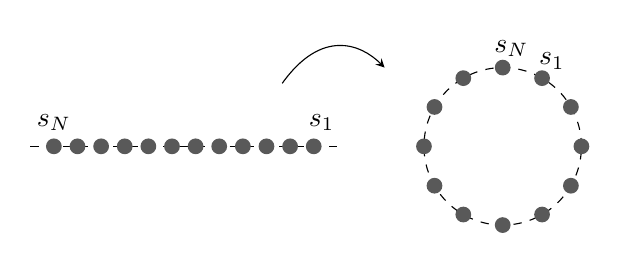
\begin{tikzpicture}
\draw[dashed] (-6,0) -- (-2,0);
\draw[variable=\x,smooth,dashed,domain=0:360,samples=360] plot (\x:1);
\foreach \i in {1,...,12}
{
	\fill[black!65!white] ({30*\i}:1) circle [radius=0.1];
	\fill[black!65!white] (-6,0) + ({0.3*\i},0) circle [radius=0.1];
}
\draw node at (85:1.25) {\(s_N\)};
\draw node at (60:1.25) {\(s_1\)};
\draw node at (-5.7,0.3) {\(s_N\)};
\draw node at (-2.3,0.3) {\(s_1\)};
\draw[>=stealth,->] (-2.8,0.8) .. controls (-2.3,1.5) and (-1.8,1.3) .. (-1.5,1);
\end{tikzpicture}
\caption{A visualisation of the physical interpretation of one-dimensional period boundary conditions: the single dimension is folded into a two-dimensional closed path. The bondary point \(s_N\) thus experiences being the neighbour of the complementary boundary point \(s_1\).}\label{fig:one_dimensional_boundary_conditions}
\end{figure}

By combining both the spin interactions and the external magnetisation, the energy of the system is given by
\begin{equation}\label{eq:Ising_system_energy}
\epsilon=-J\sum_{\expval{kl}}s_ks_l-\mu B\sum_is_i
\end{equation}
where \(\expval{kl}\) implies a summation over neighbouring spins. Note that \eqref{eq:Ising_system_energy} does not impose any particular coordinate system, in fact, the Ising model may be applied to any \(n\)-dimensional case. This project will focus on the two-dimensional case, which happens to have been solved exactly (higher-dimensional cases have not). 
\subsubsection{The \(2\times2\) system}\label{sec:2by2_system}
Assuming the system consists of four particles arranged in a square \(2\times2\) lattice, there are \(2^4=16\) number of possible arrangements of the spins \(s\). All possible microstates are sketched out in appendix \ref{app:additional_material}, the macrostates are summarised in table \ref{tab:2by2_macrostates}.
\begin{table}
\begin{tabular}{|c|c|c|}
\hline
Energy [\(J\)] & Net Spin & Degeneracy \\\hline
-8 &  4 & 1 \\\hline
0  &  2 & 4 \\\hline
0  &  0 & 4 \\\hline
8  &  0 & 2 \\\hline
0  & -2 & 4 \\\hline
-8 & -4 & 1 \\\hline
\end{tabular}
\caption{The macrostates of the \(2\times2\) Ising model system: energy \& net spin. The degeneracy refers to the number of microstates with the same macrostate.}\label{tab:2by2_macrostates}
\end{table}

Table \ref{tab:2by2_macrostates} provides a simple opportunity to evaluate various thermodynamic properties effectively. The key observation is to identify that the summation over all iterations of a variable \(A_i\) with a degeneracy \(\text{deg}(A)\) is the same as the summation over all the values of the variable \(A\) scaled with its corresponding degeneracy:
\begin{align*}
\sum_iA_i&=\big(A^1+\cdots+A^1\big)+\cdots+\big(A^n+\cdots+A^n\big)\\
&=\text{deg}(A^1)A^1+\cdots+\text{deg}(A^n)A^n\\
&=\sum_A\text{deg}(A)A
\end{align*}
where \(A\in\{A^1,\ldots,A^n\}\). The rest of this section deals with to exact evaluation of the thermodynamic properties introduced in section \ref{sec:selected_thermodynamic_properties} using this summation trick. The quantites are given a superscript \(2\times2\) to indicate that they are only valid for the \(2\times2\) Ising system.

The partition function is equal to
\begin{align}
Z^{2\times2}&=\sum_\epsilon\text{deg}(\epsilon)e^{-\epsilon\beta}\nonumber\\
&=e^{8J\beta}+4e^0+4e^0+2e^{-8J\beta}+4e^0+e^{8J\beta}\nonumber\\
&=8+2e^{-8J\beta}+2e^{8J\beta}
\end{align}

The first and second moments of the energy are therefore given by
\begin{align}
\expval{\epsilon}^{2\times2}&=\frac{1}{Z^{2\times2}}\sum_\epsilon\text{deg}(\epsilon)\epsilon\,e^{-\epsilon\beta}\nonumber\\
&=\frac{1}{Z^{2\times2}}\bigg[(-8J)e^{8J\beta}+4(0)e^0+4(0)e^0\nonumber\\
&\quad+2(8J)e^{-8J\beta}+4(0)e^0+(-8J)e^{8J\beta}\bigg]\nonumber\\
\expval{\epsilon}^{2\times2}&=\frac{16J}{Z^{2\times2}}\big(e^{-8J\beta}-e^{8J\beta}\big)\\[6mm]
\expval{\epsilon^2}^{2\times2}&=\frac{1}{Z^{2\times2}}\sum_\epsilon\text{deg}(\epsilon)\epsilon^2e^{-\epsilon\beta}\nonumber\\
&=\frac{1}{Z^{2\times2}}\bigg[(-8J)^2e^{8J\beta}+4(0)^2e^0+4(0)^2e^0\nonumber\\
&\quad+2(8J)^2e^{-8J\beta}+4(0)^2e^0+(-8J)^2e^{8J\beta}\bigg]\nonumber\\
\expval{\epsilon^2}^{2\times2}&=\frac{128J^2}{Z^{2\times2}}\big(e^{-8J\beta}+e^{8J\beta}\big)
\end{align}
which implies that the variance of the energy is
\begin{align}
\text{Var}[\epsilon]^{2\times2}&=\expval{\epsilon^2}^{2\times2}-\Big[\expval{\epsilon}^{2\times2}\Big]^2\nonumber\\
&=\frac{256J^2}{\big(Z^{2\times2}\big)^2}\bigg[\frac{Z^{2\times2}}{2}\big(e^{-8J\beta}+e^{8J\beta}\big)\nonumber\\
&\qquad\qquad\qquad-\big(e^{-8J\beta}-e^{8J\beta}\big)^2\bigg]\nonumber\\
&=\frac{512J^2}{\big(Z^{2\times2}\big)^2}\Big[Z^{2\times2}-6\Big]\label{eq:2by2_epsilon_variance}
\end{align}
\newpage
Similarly, the first and second moments of the net spin are given by
\begin{align}
\expval{M}^{2\times2}&=\frac{1}{Z^{2\times2}}\sum_\epsilon\text{deg}(\epsilon)M(\epsilon) e^{-\epsilon\beta}\nonumber\\
&=\frac{1}{Z^{2\times2}}\bigg[(4)e^{8J\beta}+4(2)e^0+4(0)e^0\nonumber\\
&\quad+2(0)e^{-8J\beta}+4(-2)e^0+(-4)e^{8J\beta}\bigg]\nonumber\\
\expval{M}^{2\times2}&=0\\[6mm]
\expval{M^2}^{2\times2}&=\frac{1}{Z^{2\times2}}\sum_\epsilon\text{deg}(M)M(\epsilon)^2e^{-\epsilon\beta}\nonumber\\
&=\frac{1}{Z^{2\times2}}\bigg[(4)^2e^{8J\beta}+4(2)^2e^0+4(0)^2e^0\nonumber\\
&\quad+2(0)^2e^{-8J\beta}+4(-2)^2e^0+(-4)^2e^{8J\beta}\bigg]\nonumber\\
\expval{M^2}^{2\times2}&=\frac{32}{Z^{2\times2}}\big(1+e^{8J\beta}\big)
\end{align}
which implies that the variance of the net spin is
\begin{align}
\text{Var}[M]^{2\times2}=\frac{32}{Z^{2\times2}}\big(1+e^{8J\beta}\big)\label{eq:2by2_netspin_variance}
\end{align}

Furthermore, the expected magnetisation \(|M|\) is
\begin{align}
\expval{|M|}^{2\times2}&=\frac{1}{Z^{2\times2}}\sum_{\epsilon}\text{deg}(\epsilon)|M(\epsilon)|\,e^{-\epsilon\beta}\nonumber\\
&=\frac{1}{Z^{2\times2}}\bigg[|4|e^{8J\beta}+4|2|e^0+4|0|e^0\nonumber\\
&\quad+2|0|e^{-8J\beta}+4|-2|e^0+|-4|e^{8J\beta}\bigg]\nonumber\\
\expval{|M|}^{2\times2}&=\frac{1}{Z^{2\times2}}\big(16+4e^{8J\beta}\big)
\end{align}

The heat capacity \(C_V^{2\times2}\) and the magnetic susceptibility \(\chi^{2\times2}\) are found using equations \eqref{eq:heat_capacity} and \eqref{eq:magnetic_sucseptibility} respectively (they are essentially a rescaling of the energy and net spin variances). Plots of \(C_V^{2\times2}\) and \(\chi^{2\times2}\) are included in appendix \ref{app:additional_material}.
\subsubsection{The critical point}
The Ising model exhibits a magnetic phase transition for 2- or higher-dimensional systems. This phase transition is characterised by a so-called critical point at which thermodynamic quantities typically diverge/converge to zero or experience an abrupt restructuring of their behaviour. The two-dimensional system without an external magnetic field has been solved exactly (see \cite{Onsager}), which will serve as a great benchmark for simulations. The analytical solution finds that the critical tempearture for which the phase transition takes place is:
\begin{equation}
\frac{k_BT_C}{J}=\frac{2}{\ln\big(1+\sqrt{2}\big)}\cong2.269
\end{equation}

For temperatures close to the critical temperature, the thermodynamic quantities behave according to a power law. Most prominently, the net magnetisation, heat capacity and magnetic susceptibility behave according to:
\begin{subequations}\label{eq:exact_power_laws}
\begin{align}
\expval{M(T)}&\propto(T-T_C)^\beta\\
C_V(T)&\propto|T-T_C|^\alpha\\
\chi(T)&\propto|T-T_C|^\gamma
\end{align}
\end{subequations}
where \(\beta\), \(\alpha\) and \(\gamma\) are examples of \emph{"critical exponents"}. The analytical solution shows that these exponents for the unperturbed two-dimensional system are:
\[\beta=\frac{1}{8}\qc\alpha=0\qand\gamma=\frac{7}{4}\]

The phase transition is said to be "magnetic" because the magnetic properties of the system are abruptly altered. However, this name is misleading as the magnetic properties are uniquely defined by the system's underlying spin-configuration. The system's true transition is the movement from an ordered state, in which the spins are mostly aligned, to a disordered state, in which the spins adapt random values. The ordered state (with \(T\leq T_C\)) exhibits spontaneous magnetisation, meaning \(\expval{M}\neq0\), while the disordered state (with \(T\geq T_C\)) does not. That is, \(\expval{M}\) should be nonzero for \(T\leq T_C\) and approximately zero otherwise. 

Another important feature of the critical point is the correlation length \(\xi\):
\begin{equation}
\xi(T)=|T-T_C|^{-\nu}
\end{equation}
where \(\nu\) is another critical exponent whose analytical solution in the unperturbed two-dimensional system is \(\nu=1\). The correlation length is essentially a measure of the orderedness of a system, in particular, a measure of repetititiveness. With regards to the Ising model, this can be interpreted as a mesaure of whether spins are aligned or not. The correlation function diverges as \(T\) approach \(T_C\).

Because this project will employ period boundary conditions instead of an infinitely sized lattice,\footnote{As if there was a choice.} there is necessarily a small deviation in the critical temperature experienced by the finite lattice and the infinite lattice. This deviation can actually be theoretically predicted using finite size scaling:
\begin{equation}\label{eq:ideal_critical_temperature_scale}
T_C(L)-T_C=aL^{-1/\nu}
\end{equation}
where \(L\) is the number of spins along the side of an \(L\times L\) lattice and \(a\) is a constant. Furthermore, equations \ref{eq:exact_power_laws} will also experience a similar deviation:
\begin{subequations}\label{eq:scaled_power_laws}
\begin{align}
\expval{M(T)}&\to L^{-\beta/\nu}\\
C_V(T)&\to L^{\alpha/\nu}\\
\chi(T)&\to L^{\gamma/\nu}
\end{align}
\end{subequations}
where \(T\) is close to \(T_C(L)\).


\subsection{Numerical Simulations}
The following theory is based partially on the FYS 3150 lecture notes on Monte Carlo methods \cite{montecarlo_lec_notes} and statistical physics \cite{statphys}, and notes on Monte Carlo integration by Dave Edwards \cite{montecarlo_Edwards}.
\subsubsection{Monte Carlo integration}
In the field of numerical integration, one of the most common strategies is so-called Monte Carlo integration. Monte Carlo integration cleverly exploits the properties of stochastic variables and probability theory by rewriting the problem in terms of expected values. The basic problem is to integrate a scalar integral on the form
\begin{equation}\label{eq:general_integral}
I=\int_D\dd{x}f(x)
\end{equation}
where \(x\in D\) is not necessarily one-dimensional. Let \(p(x)\) denote a particular known distribution and consider the following change of variables:
\begin{equation}\label{eq:integral_to_expected_value}
\int_D\dd{x}f(x)=\int_{x\in D}\dd{p(x)}\,\frac{f(x)}{p(x)}
\end{equation}
That is, the integral \(I\) is equal to the expected value of \(f(x)/p(x)\) with respect to the probability distribution \(p(x)\). The idea is to draw \(N_\text{MC}\) random numbers \(X\sim p(x)\) and estimate the expected value with the sample expected value:
\begin{equation}\label{eq:approximated_expected_value}
\expval{\frac{f(x)}{p(x)}}_X\approx\sum_{i=1}^{N_\text{MC}}\frac{f(x_i)}{p(x_i)}p(x_i)=\sum_{i=1}^{N_\text{MC}}f(x_i)
\end{equation}
which becomes an equality when \(N_\text{MC}\to\infty\) due to the Law of Large Numbers.

Although \eqref{eq:approximated_expected_value} is exact in the large-\(N_\text{MC}\) limit, the choice of \(p(x)\) may affect the lower boundary of \(N_\text{MC}\) for which the sample expected value is fairly accurate. Hence, choosing \(p(x)\) is an important component of the design of a Monte Carlo integration. The simplest choice of \(p(x)\) is the uniform distribution, which sadly is particularly unstable for \(f(x)\) functions with sharp peaks.

Effective algorithms that a large number of computations of \(p(x)\) have been developed, one of which is presented below. Nonetheless, the basic foundation for any Monte Carlo integration techinque is summarised by the following algorithm.
\begin{algorithm}[H]
\caption{Standard Monte Carlo Integration}\label{algo:standard_Monte_Carlo}
\begin{algorithmic}[1]
\State Define \(N_\text{MC}\).
\State Initialise \(\text{SUM}=0\).
\NoDoFor {\(i=1,\ldots,N_\text{MC}\):}
	\State Draw \(x_i\) at random according to \(p(x)\).
	\State Evaluate \(f(x_i)\).
	\State Add contribution: \(\text{SUM}\mathrel{{+}{=}}f(x_i)\)
\EndFor
\State Normalise final value: \(I=\text{SUM}/N_\text{MC}\).
\end{algorithmic}
\end{algorithm}

\subsubsection{Markov chains}
A Markov chain is a stochastic model for the discrete evolution \footnote{A Markov chain may be generalised to continuous evolution, but this will not be used in this project.} of a so-called "memoryless system". In this context, to be memoryless implies that each step is only dependent on the previous state of the system (i.e., the system does not conserve memory of earlier states). A common usage of Markov chains is to mimick time evolution, but this is just an example.

In its most general form, a (discrete) Markov chain is a sequence of random variables \(X_1,X_2,\ldots\), which satisfy the Markov property. Simplified, the Markov property requires that the probability of moving from a state \(X_n\) to state \(X_{n+1}\) is only dependent on \(X_n\). The state space may either be continuous or discrete, each of which invoke a distinct, albeit similar, formalism. Because the Boltzmann distribution is a continuous distribution, the discrete formalism will be ignored in favour of the continuous.

Say the state space for a particular Markov chain is \(\mathcal{S}\), then a \emph{stochastic kernel} on \(\Sspace\) is a function \(p:\Sspace\times\Sspace\to\mathbb{R}\) that satisfies
\[p(x,y)\leq0,\,\forall x,y\in\Sspace\qand\int_\Sspace\dd{y}p(x,y)=1,\,\forall x\in\Sspace\]
Each Markov chain is parametrised by its corresponding stochastic kernel, which in this sense is usually referred to as the transition probability density. Now for every \(p(x,y)\) there exists a so-called \emph{Markov operator} \(P\) that is such that
\[\big[(\cdot)P\big](y)=\int_\Sspace\dd{x}p(x,y)(\cdot)\]
Note in particular that \(P\) is a left-acting operator, as per usual in the literature.

Furthermore, say the Markov chain has continued for \(n\) steps with previous measurements \(X_1=x_1,X_2=x_2,\ \cdots,X_n=x_n\), then the next measurement \(X_{n+1}=y\) is drawn according to the distribution \(p^{(n+1)}(x)\) whose evolution from the current distribution \(p^{(n)}(x)\) is given by the Markov operator of the Markov chain:
\begin{equation}\label{eq:Markov_Chain_next_distribution}
p^{(n+1)}(y)=\big[p^{(n)}(x)P\big](y)=\int_\Sspace\dd{x}p(x,y)p^{(n)}(x)
\end{equation}

A special case of \eqref{eq:Markov_Chain_next_distribution} is when the distribution is invariant of \(P\), that is, when \(p^{(n+1)}=p^{(n)}\). This behaviour is called a stationary distribution and is usually denoted by \(\pi(x)\):\footnote{Becuase choosing \(\pi\) to represent something else other than \(\pi\) seemed like a great idea, obviously.}
\begin{equation}
\pi(y)=\int_\Sspace\dd{x}p(x,y)\pi(x)
\end{equation}
Such a state is guaranteed if the Markov chain obeys the so-called \emph{detailed balance} condition. Provided a transition probability density \(p(x,y)\) and a particular distribution \(\pi(x)\), then the detailed balance condition states that the Markov chain corresponding to \(p(x,y)\) is \emph{reversible} with respect to \(\pi(x)\) if
\begin{equation}\label{eq:Markov_Chain_detailed_balance}
\pi(x)p(x,y)=\pi(y)p(y,x),\ \forall x,y\in\Sspace
\end{equation}
It follows that
\[\int_\Sspace\dd{x}p(x,y)\pi(x)=\pi(y)\int\dd{x}p(y,x)=\pi(y)\]
because \(p(x,y)\) is normalised for all \(x,y\in\Sspace\). In conclusion, in case a Markov chain is "well-behaved", meaning it satisfies detailed balance, the so-called \emph{limiting distribution} of the Markov chain approaches \(\pi\) as \(n\to\infty\):
\begin{equation}
\lim_{n\to\infty}\big[p^{(0)}(x)P^n\big](y)=\pi(y)
\end{equation}
where \(P^n\) implies repeated operations on \(p^{(0)}\), \(p^{(1)}\), etc.
\subsubsection{Markov Chain Monte Carlo: The Metropolis algorithm}
As the name implies, Markov Chain Monte Carlo (MCMC) methods combine the concept of a Markov chain with Monte Carlo methods. There exists several MCMC methods, each with unique properties that may or may not be benefitial. This project will focus on the so-called \emph{Metropolis} algorithm, which is a special case of the \emph{Metropolis-Hastings} algorithm.

The basic idea behind the MCMC methods stems from equation \eqref{eq:approximated_expected_value}. Ideally one would be able to draw a sufficiently large number of states \(x\) from \(p(x)\) and follow algorithm \ref{algo:standard_Monte_Carlo} religiously. However, this is incredibly computation-ineffective and essentially infeasible for a standard compute. Enter Markov chains: A Markov chain with limiting distribution \(\pi(x)=p(x)\) would necessarily generate states that are approximately distributed according to \(p(x)\). It turns out that this may be exploited in order to avoid large computations.

The mathematics of MCMC methods are based on the detailed balance principle, consider the following rearranging of equation \eqref{eq:Markov_Chain_detailed_balance}:
\[\frac{p(x,y)}{p(y,x)}=\frac{\pi(y)}{\pi(x)}\]
Now, suppose the current state of the Markov chain governed by \(p(x,y)\) is \(X_n\), i.e., the \(n^\text{th}\) state in the chain. The idea is to separate the transition process into two steps: an initial \emph{proposal}, and an \emph{acceptance/rejection} step. These steps should be independent so that probability is independent, meaning the probability density of proposing a state \(y\), \(g(y|x)\), is independent of the probability of accepting the proposal, \(\alpha(x,y)\). Because they are independent, it follows that
\begin{equation}
p(x,y)=g(y|x)\alpha(x,y)
\end{equation}
meaning the above criteria may be rewritten as
\begin{equation}\label{eq:MCMC_detailed_balance_with_TandA}
\frac{\alpha(y,x)}{\alpha(x,y)}=\frac{p(y)}{p(x)}\frac{g(x|y)}{g(y|x)}
\end{equation}
where \(p(x)=\pi(x)\) is the assertion of MCMC methods that the limiting distribution of the Markov chain governed by \(p(x,y)\) is the integrand of equation \eqref{eq:general_integral}. This expression is particularly easy to implement in case the normalisation of \(p\) and \(g\) are independent on \(x\) and \(y\), or if they happen to cancel each other (although this is very unlikely).

The last step it to choose an acceptance probability \(\alpha(y,x)\) that satisfies \ref{eq:MCMC_detailed_balance_with_TandA}, the \emph{Metropolis choice} is
\begin{equation}\label{eq:Metropolis_Hastings_acceptance_probability}
\alpha(y,x)=\min\left\lbrace 1,\frac{p(y)}{p(x)}\frac{g(x|y)}{g(y|x)}\right\rbrace
\end{equation}
The Metropolis-Hastings algorithm may now be stated:
\begin{algorithm}[H]
\caption{The Metropolis-Hastings Algorithm}\label{algo:Metropolis_Hastings}
\begin{algorithmic}[1]
\State Initialise the first state \(X_0\).
\NoDoFor {\(n=1,\ldots,N_\text{MH}\):}
	\State Generate a proposal \(y\) according to \(g(y|x)\).
	\State Evaluate acceptance probability \(\alpha(y,x)\).
	\NoThenIf {\(\alpha(y,x)=1\):}
		\State Accept \(y\).
	\Else
		\State Draw a uniformly distributed number \(a\in[0,1]\).
		\NoThenIf {\(a\leq\alpha(y,x)\):}
			\State Accept \(y\).
		\Else
			\State Reject \(y\) and set \(X_{n+1}=X_n\).
		\EndIf
	\EndIf
\EndFor
\end{algorithmic}
\end{algorithm}
where \(N_\text{MH}\) is the number of steps in the Markov chain. Note that the algorithm above does not factor in the Monte Carlo update, this is because the central purpose of the Metropolis-Hastings algorithm is namely just to sample \(x\) values according to \(p(x)\). Nonethelesss, implementations of the algorithm usually include an intermediate step inside this loop in order to avoid multiple loops.

Furthermore, although the distribution is guaranteed to converge, it does not necessarily converge within the first few steps. Accordingly, a common practice is to perform \(N_\text{prep}\) preparation updates to \(X_0\) in a process known as "burn-in", before invoking the Monte Carlo steps. When a step in the Markov chain represents a forward step in time, the amount of necessary burn-in is commonly referred to as the equilibration time of the system.

As previously mentioned, this project will implement the Metropolis algorithm, which is a special case of the Metropolis-Hastings algorithm. The Metropolis assumes that \(g\) is symmetric in \(x\) and \(y\), meaning \(g(x|y)=g(y|x)\). This implies that the acceptance probability may be simplified to
\begin{equation}\label{eq:Metropolis_acceptance_probability}
\alpha_\text{M}(y,x)=\min\left\lbrace1,\frac{p(y)}{p(x)}\right\rbrace
\end{equation}
\section{Method}
The main focus of this project is to study the two-dimensional Ising model, where the overaching goal is to estimate the critical temperature for the magnetic phase transition. The system is assumed to be under no influence from external magnetic fields such that the phase transition is completely dependent on unperturbed system. The time-evolution of the system is modelled using a Markov chain, where each step represents a small increment in time. In order to study the critical temperature, the mean magnetisation, heat capacity and magnetic susceptibility will be studied as functions of temperature. The resulting integrals will be estimated using Monte Carlo simulations with Metropolis-sampled states.

Before continuing to the numerical experiments of this project, the following section will describe some general aspects of the simulation.
\subsection{The Simulation - General Aspects}
The Ising system is parametrised by temperature via \(\beta=1/k_BT\), which is assumed to be constant during the simulation. To goal is to estimate a series of expectance values as functions of temperature, meaning various integrals must be estimated using Monte Carlo methods. The energy of the ideal Ising model (infinitely large lattice) is continuous with respect to temperature, this will be approximated using periodic boundary conditions such that the continuous formalism developed above is applicable, in particular the Metropolis algorithm. This project will not study the effects of irregular lattices and will therefore use a square lattice with \(L\times L\) spins.
\subsubsection{The basic approach - Flip one spin}
The (micro-)state of the Ising system is the spin configuration of the lattice structure. Becuase the Ising system is canonical, the energy must necessarily behave according to the Boltzmann distribution (equation \eqref{eq:Boltzmann_Distribution}). Now, assuming \(g\) is symmetric in \(x\) and \(y\), it follows that the Metropolis acceptance probability is equal to
\begin{align}
\alpha(y,x)&=\min\left\lbrace1,\frac{\frac{1}{Z}e^{-\epsilon(y)\beta}}{\frac{1}{Z}e^{-\epsilon(x)\beta}}\right\rbrace\nonumber\\
&=\min\left\lbrace1,e^{[\epsilon(x)-\epsilon(y)]\beta}\right\rbrace\label{eq:Ising_Metropolis_acceptance}
\end{align}
However, the exponential may further simplified using a clever choice of \(g\). The approach is sometimes called the \emph{"flip one"} tactic. The idea is to assume that \(g\) is only nonzero for the states that are different from \(x\) by a single spin-permutation (i.e. a single spin flip). At its face, this imposes no significance on the exponential in \(\alpha(y,x)\). However, observe that with a single spin flip, the only difference between \(x\) and \(y\) are the interactions between the flipped spin and its neighbours (see figure \ref{fig:flip_one_tactic}). This implies that to evaluate the change in energy and net magnetisation between \(x\) and \(y\), only the flipped interactions have to be considered. The possible arrangements of the flipped spin and its neighbours are shown in appendix \ref{app:additional_material}.

\begin{figure}
\centering
\scalebox{1.5}{
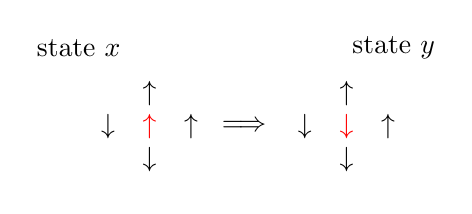
\begin{tikzpicture}
\draw node at (0,0) {\spinconfigmatrixneighbours{\ua}{\da}{{\color{red}\ua}}{\ua}{\da}};
\draw node at (1.2,0) {\(\implies\)};
\draw node at (2.5,0) {\spinconfigmatrixneighbours{\ua}{\da}{{\color{red}\da}}{\ua}{\da}};
\draw node at (-0.9,1) {state \(x\)};
\draw node at (3.1,1) {state \(y\)};
\end{tikzpicture}}
\caption{An example transition from state \(x\) to state \(y\) using the flip one tactic. The only difference is the flipped red spin, the rest of the spin configuration remains the same.}\label{fig:flip_one_tactic}
\end{figure}

Without a external magnetic field (\(B=0\)), the energy difference is
\begin{align*}
\epsilon(y)-\epsilon(x)&=-J\sum_{\expval{kl}}s_k(y)s_l(y)+J\sum_{\expval{kl}}s_k(x)s_l(x)
\end{align*}
where \(s_k(x)\) denotes the spin at label \(k\) in state \(x\). Each of these sums may be divided into two components: one containing the flipped spin interactions and the rest:
\[\sum_{\expval{kl}}s_k(\cdot)s_l(\cdot)=\sum_{\expval{ki}}s_k(\cdot)s_i(\cdot)+\sum_{\expval{kl}\,\wedge\,l\neq i}s_k(\cdot)s_l(\cdot)\]
where \(i\) denotes the flipped spin. The two "rest" sums cancel and, as \(s_k(x)=s_k(y)=s_k\), one finds that:
\[\epsilon(y)-\epsilon(x)=-J\sum_{\expval{ki}}s_k\big(s_i(y)-s_i(x)\big)\]
Furthermore, the flipped spin necessarily satisfies \(s_i(y)=-s_i(x)\), meaning \(s_i(y)-s_i(x)=-2s_i(x)\). In conclusion,
\begin{equation}\label{eq:Ising_flip_one_energy_change}
\epsilon(y)-\epsilon(x)=\Delta\epsilon=2Js_i(x)\sum_{\expval{k(i)}}s_k
\end{equation}
where \(\expval{k(i)}\) denotes summation over the neighbours \(k\) of \(i\), but not including \(i\). Because there is a limited number of possible flip-one arrangements, there is thus only a limited number of possible values for \(\epsilon(y)-\epsilon(x)\). This is important because it allows for the computation of the exponential in \eqref{eq:Ising_Metropolis_acceptance} outside the Metropolis loop. More on this below.

To obtain the change in net magnetisation, the same approach is followed: The total sums are divided into a flipped sum and a rest sum. However, because the net magnetisation does not loop over neighbours, the flipped sum reduces to the single flipped spin:
\[M(y)-M(x)=\sum_{j}s_j(y)-\sum_{j}s_j(x)=s_i(y)-s_i(x)\]
where \(j\) loops over all spins, while \(i\) denotes the flipped spin. Again, as \(s_i(x)=-s_i(y)\) it follows that
\begin{equation}
M(y)-M(x)=\Delta M=2s_i(y)
\end{equation}

\subsubsection{The algorithm}
The algorithm is basically a special case of the combination of algorithms \ref{algo:standard_Monte_Carlo} and \ref{algo:Metropolis_Hastings}. Nonetheless, some minor details (such as evaluating the exponential outside the Monte Carlo simulation) have been implemented to spare computation. Further adjustments or additions to the algorithm are introduced where relevant, however the general algorithm is:
\begin{algorithm}[H]
\caption{The Ising Model Metropolis Monte Carlo}\label{algo:Ising_Model_Algorithm}
\begin{algorithmic}[1]
\State Define \(N_\text{MC}\), \(T\) and \(L\).
\State Initialise Monte Carlo integrals.
\State Precompute all possible \(\exp(-\Delta\epsilon\beta)\).
\State Initialise \(L\times L\) spin state matrix.
\State Initialise state energy and net magnetisation.
\NoDoFor {\(n=1,\ldots,N_\text{MC}\):}
	\NoDoFor {\(k=1,\ldots,L\):}
		\NoDoFor {\(l=1,\ldots,L\):}
			\State Generate random index \(i\in\{1,\ldots,L\}\).
			\State Generate random index \(j\in\{1,\ldots,L\}\).
			\State Propose new state \(y\) with spin \(s_{ij}\) flipped.
			\State Evaluate net magnetisation of \((i,j)\) neighbours.
			\State Infer \(\alpha=\exp\big(-\Delta\epsilon\beta\big)\).
			\State Draw \(a\sim\mathcal{U}(0,1)\).
			\NoThenIf {\(a\leq\alpha\):}
				\State Accept \(y\): Flip spin \((i,j)\) in state matrix.
				\State Update state energy and net magnetisation.
			\EndIf
		\EndFor
	\EndFor
	\State Add contribution to Monte Carlo integrals.
\EndFor
\State Normalise Monte Carlo integrals according to \(N_\text{MC}\) and \(L\times L\).
\end{algorithmic}
\end{algorithm}
There are several components of algorithm \ref{algo:Ising_Model_Algorithm} that are implemented for computational reasons, these are explained below. On a different note, observe the triple \texttt{for}-loop in \ref{algo:Ising_Model_Algorithm}: this is actually a double loop in disguise. The outer loop is the standard Monte Carlo integration loop from algorithm \ref{algo:standard_Monte_Carlo}. The two inner loops (\(k\) and \(l\)) are actually the single Metropolis loop in algorithm \ref{algo:Metropolis_Hastings}. The idea it to loop over every spin in the lattice in order to produce an uncorrelated new state. However, flipping every spin in the lattice would just return the inverse (negative) state, thus each spin is chosen at random.

As equation \eqref{eq:Ising_Metropolis_acceptance} illustrates, the only factor with an impact on \(\alpha(y,x)\) (and thereby the probability of acceptance) is \(\epsilon(y)-\epsilon(x)\), which equation \eqref{eq:Ising_flip_one_energy_change} indicates is uniquely determined by the flipped spin and its neighbours. Moreover, because there is a limited number of possible arrangements for the neighbours of the flipped spin, there is thus a limited number of \(\alpha(y,x)\). This observation is implemented in algorithm \ref{algo:Ising_Model_Algorithm} in lines 3 and 13: because \eqref{eq:Ising_flip_one_energy_change} is an integer number of \(J\), this integer uniquely determines \(\alpha(y,x)\) by acting as an index for the array of possible \(\alpha(y,x)\) values that is computed before the iteration.

Furthermore, note that the Metropolis-Hastings algorithm (\ref{algo:Metropolis_Hastings}) contains a two-step \texttt{if}-test. In particular, the algorithm computes first \(\alpha=\exp(-\Delta\epsilon\beta)\) and then evaluates \(\alpha(y,x)\). In case \(\alpha\) is greater than 1, the move is directly accepted. On the other hand, if \(\alpha\) is the smaller of the two, the move is accepted with probability \(\alpha\) by comparing it with a random number \(a\sim\mathcal{U}(0,1)\). 


\subsection{Numerical Experiments}
The following section describes the numerical experiments that are studied in this project. There are 4 experiments in total, each serving a unique task. The culmination of the project is (of course) experiment no. 4 in which the goal is to estimate the critical temperature of the magnetic phase transition.

All experiments will use a scaled tempearture with units \((J/k_B)\) K, meaning both \(J\) and \(k_B\) are essentially removed from all equations.
\subsubsection{Experiment 1: Verifying the computations}
To begin the project, the Ising simulation will be compared to the known \(2\times2\) system with a temperature of \(T=1\). The thermodynomic properties of interest to this experiment are: \(\expval{\epsilon}\), \(\expval{\epsilon^2}\), \(\expval{M}\) and \(\expval{M^2}\) whose analytic solutions are:
\[\expval{\epsilon}^{2\times2}\cong-1.9973\qc\expval{\epsilon^2}^{2\times2}\cong15.979\]
\[\expval{M}^{2\times2}\cong0\qc\expval{M^2}^{2\times2}\cong3.9960\]

The main goal of this experiment is to verify that the Metropolis algorithm is succesful in its random sampling of states by making a crude analysis of the Monte Carlo simulations' dependency on the number of Monte Carlo cycles \(N_\text{MC}\). To simplify, the Metropolis algorithm is given zero burn-in time, meaning all cycles contribute towards the integrals. The experiment will be run 40 unique times for each of the following number of Monte Carlo cycles: \(10^2\), \(10^3\), \(10^4\), \(10^5\), \(10^6\) and \(10^7\).
\subsubsection{Experiment 2: Studying the burn-in}
The next experiment will focus on the Monte Carlo burn-in with special interest on the number of sufficient cycles and the importance of the initial state. The experiment features a \(20\times20\) lattice with either of two initial states: the ground state (ordered) and a random state (disordered). In the ground state (lowest energy state), all spins point upwards (see equation \eqref{eq:Ising_system_energy}), whereas in the random state, all spins are equally distributed between down and up spins.

The jist of the experiment is to perform the simulation as in experiment 1, however track the contributions to the Monte Carlo integrals throughout the simulation. The resulting arrays, which contain the commulative sums of the integration, are then normalised according to the number of cycles that has passed. The experiment will use an upper boundary of \(N_\text{MC}=10^6\) for all runs. Moreover, the experiment will also be run with 3 different temperatures: \(T=1.0\), \(T=1.7\) and \(T=2.4\) in order to study temperature dependence.

To summarise, the experiment is run with \(N_\text{MC}=10^6\) for 3 different temperatures starting from 2 dfferent initial states, making a total 6 different runs. In addition to the Monte Carlo integrals, this experiment will also track how the number of accepted proposals evolves with increasing number of Monte Carlo cycles.
\subsubsection{Experiment 3: The energy-distribution: A frequentist approach}
Having found a sufficient burn-in equilibriation time, the next step is to study the established equilibrium as it continues to evolve. To do so, the focus falls on the energy-distribution of the spin-states produced by the Metroplis algorithm (after converging). This distribution will be determined using a frequentist approach by measuring (counting) the frequency of each energy as the system evolves (recall that the energy can only make integer steps of \(J\)).

Similar to the previous experiment, this experiment will also use a lattice with features \(20\times20\) and be run with temperatures \(T=1.0\), \(T=1.7\) and \(T=1.4\). The system is initialised from the ground state and given a burn-in based on the equilibration time found in the previous experiment. Starting from the equilibrium state, the system is simulated over \(10^6\) steps in order to provide a decent sample size. Particular interest is placed on how the spread in the energy (during evolution) behaves with respect to the temperature of the system.

The Boltzmann distribution is a gaussian with respect to energy, meaning the resulting distributions should ideally be bell-curves.
\subsubsection{Experiment 4: Studying the phase transition}
The final experiment in this project is to study the phase transition of the Ising system as a function of the number spins \(L\) in the \(L\times L\) lattice. In comparison with the other experiments, this experiment is by far the most computationally heavy. Thus, only a handful of \(L\) values will be used. Furthermore, the analytical critical temperature is about 2.27, so the simulations will use a focused temperature region of \(T\in[2.23,2.31]\) in order to capture the more details regarding the transition.

The simulations will use \(10^6\) cycles for both the burn-in and the Monte Carlo integration. Furthermore, the system is initialised from the ground state with 25 linearly spaced temperatures between and including 2.23 and 2.31. All simulations are run for \(L=40\), \(L=60\), \(L=80\) and \(L=100\). In order to save time, resources and MC cycles, the computation will be implemented using parallel programming. In particular, using Open MPI, the temperature range is divided into four equally large regions and simulated simultaneously.

The thermodynamic quantities of interest to this experiment are: \(\expval{\epsilon}\), \(\expval{|M|}\), \(C_V\) and \(\chi\) as functions of temperature. Although the definition of \(\chi\) uses \(\expval{M}\), its value will be evaluated using \(\expval{|M|}\) in order to regularize fluctuations. 

Finally, the critical temperature will be estimated using either of equations \eqref{eq:scaled_power_laws} (the choice depends on the experimental results) and a suiting polynomial fit. Having found the critical temperatures, the final estimate of the ideal critical temperature is found using \eqref{eq:ideal_critical_temperature_scale} (the ideal \(T_C\) is the \(1/L\to0\) intercept of the \(T_C(L)\) curve).

\section{Results}
\subsection{Experiment 1}
The experiments showed a clear tendency for inaccurate estimates when the number of Monte Carlo cycles dropped below \(\approx10^6\). Figure \ref{fig:2by2_expected_netmagnetisation} shows a plot of the expected net magnetisation a function of the number of Monte Carlo cycles for different runs. The mean estimate clearly approach 0 (the analytical solution) with increasing \(N_\text{MC}\), indicating that the algorithm successfully simulating the Ising model. This is further supported by the decreasing spread of the estimates as \(N_\text{MC}\) increases. Table \ref{tab:results_experiment1} shows a comparison between the exact expectance values \(\expval{\epsilon},\ldots,\expval{M^2}\) and the \(N_\text{MC}=10^7\) estimates. The estimates are incredibly accurate with a relative error of only \(\approx0.06\)\%, even without a burn-in period.

All indicators point towards the algorithm being successful in its simulation of the Ising model.

\begin{figure}[hb]
\centering
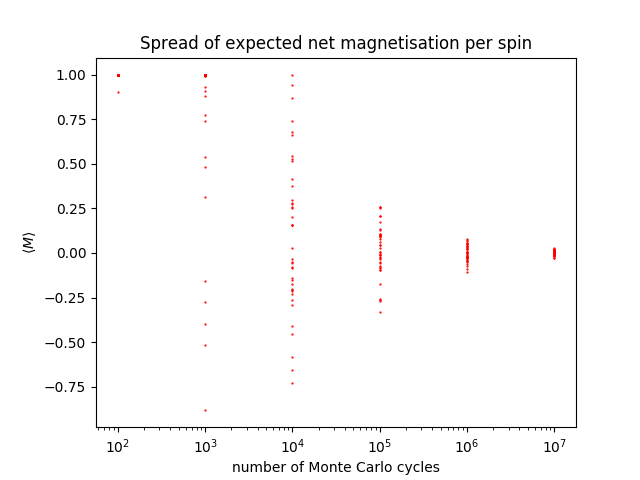
\includegraphics[scale=0.5]{../output/figures/experiment1/netmagnetisation.png}
\caption{Estimates of the expected net magnetisation for the \(2\times2\) Ising system with \(T=1\). The analytic value is 0, which the graph shows a clear tendency towards.}\label{fig:2by2_expected_netmagnetisation}
\end{figure}

\begin{table}[hb]
\centering
\begin{tabular}{|c|c|c|c|c|}
\hline\rule{0pt}{0.3cm}
& \(\expval{\epsilon}\) & \(\expval{\epsilon^2}\) & \(\expval{M}\) & \(\expval{M^2}\) \\\hline
exact & -1.997 & 15.979 & 0.000 & 3.996 \\\hline\rule{0pt}{0.4cm}
best run & -1.996 & 15.968 & \(1.5856\cdot10^{-3}\) & 3.993 \\\hline\rule{0pt}{0.4cm}
relative error [\%] & 0.05 & 0.07 & N/A & 0.08 \\\hline
\end{tabular}
\caption{Comparison between the exact solution and the best numerical result for the \(2\times2\) Ising system. The relative error is computed using \((\text{true}-\text{estimate})/\text{true}\). The error of \(\expval{M}\) is not included due to division by zero.}\label{tab:results_experiment1}
\end{table}
\newpage
\subsection{Experiment 2}
The results from the experiment are shown in figures \ref{fig:experiment2_energy}-\ref{fig:experiment2_accepted}. Generally speaking, the low temperature simulations (red and green graphs) show a much more stable tendency towards their equilibrium states, whereas the high-temperature simulation (blue graphs) shows a slightly more rugged path. Figure \ref{fig:experiment2_accepted} shows the accumulated number of accepted proposals througout the simulation, and most notably shows that all simulations have approximately constant acceptance rates. It is interesting that even the high-temperature simulation shows this behaviour as opposed to showing a decreasing rate of acceptance when equilibrium is established. It points towards an equilibrium state with a strong tendency for fluctuations, albeit too small to break the equilibrium.

In addition, the high-temperature simulation converges on the stable equilibrium at a much later time than the low-temperature simulations. Nonetheless, all systems show equilibrium behaviour after some \(10^5\) Monte Carlo cycles.

Another interesting detail is that the initial state seems to have no significant impact on the convergence to the equilibrium state. This is especially interesting in the high-temperature case because it signifies that extra care with the initial state is not necessary in future experiments.


\begin{figure}
\centering
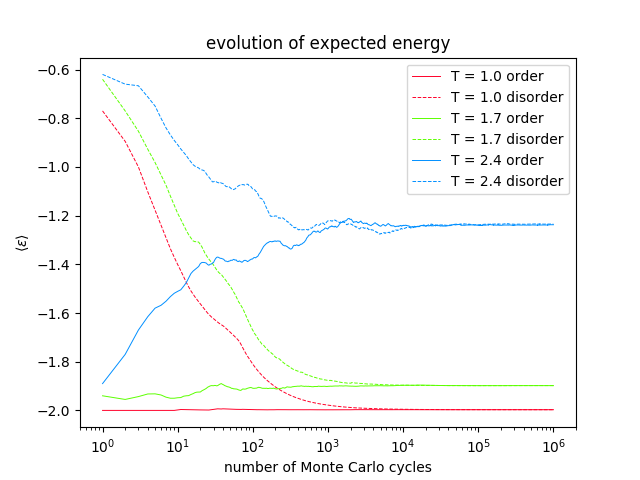
\includegraphics[scale=0.5]{../output/figures/experiment2/energy.png}
\caption{Evolution of \(\expval{\epsilon}\) of the \(20\times20\) Ising system.}\label{fig:experiment2_energy}
\end{figure}

\begin{figure}
\centering
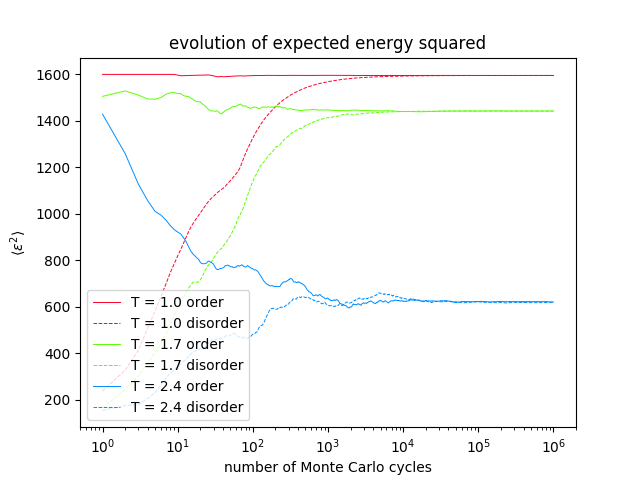
\includegraphics[scale=0.5]{../output/figures/experiment2/energy2.png}
\caption{Evolution of \(\expval{\epsilon^2}\) of the \(20\times20\) Ising system.}\label{fig:experiment2_energy2}
\end{figure}

\begin{figure}
\centering
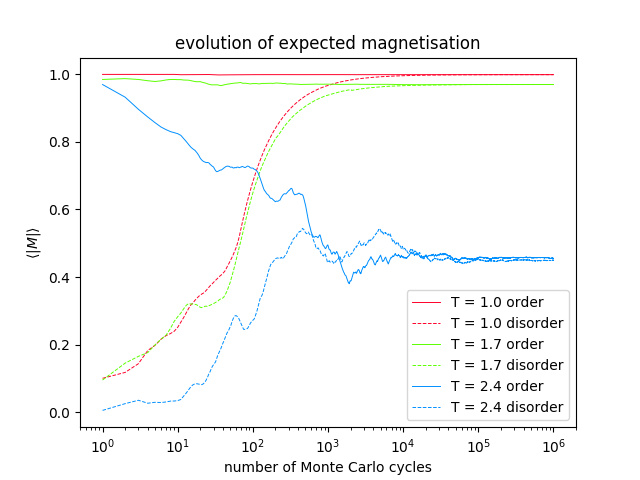
\includegraphics[scale=0.5]{../output/figures/experiment2/magnetisation.png}
\caption{Evolution of \(\expval{|M|}\) of the \(20\times20\) Ising system.}\label{fig:experiment2_magnetisation}
\end{figure}

\begin{figure}
\centering
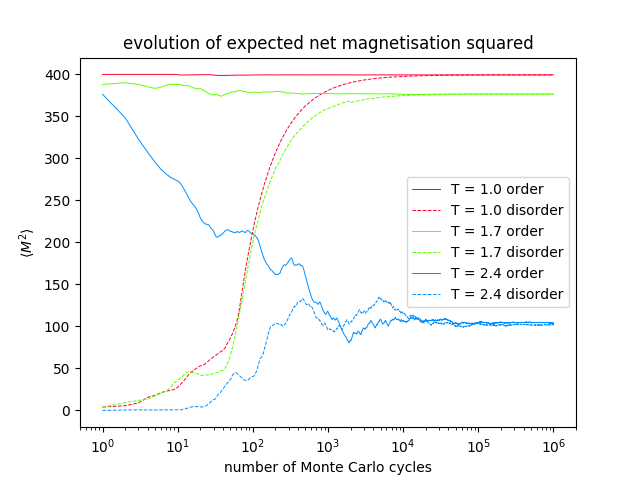
\includegraphics[scale=0.5]{../output/figures/experiment2/netmagnetisation2.png}
\caption{Evolution of \(\expval{M}\) of the \(20\times20\) Ising system.}\label{fig:experiment2_netmagnetisation}
\end{figure}

\begin{figure}
\centering
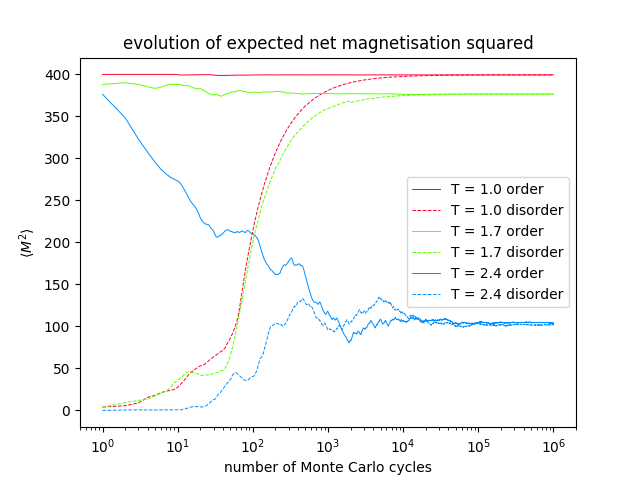
\includegraphics[scale=0.5]{../output/figures/experiment2/netmagnetisation2.png}
\caption{Evolution of \(\expval{M^2}\) of the \(20\times20\) Ising system.}\label{fig:experiment2_netmagnetisation2}
\end{figure}

\begin{figure}
\centering
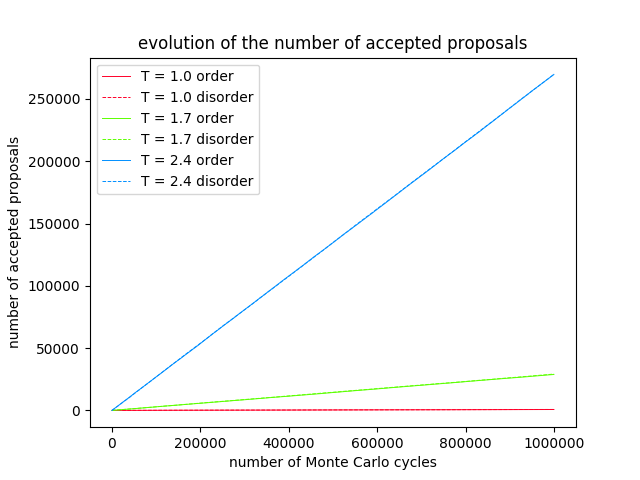
\includegraphics[scale=0.5]{../output/figures/experiment2/accepted.png}
\caption{Number of accepted proposals from the Metropolis algorithm in the evolutino of the \(20\times20\) Ising system.}\label{fig:experiment2_accepted}
\end{figure}

\subsection{Experiment 3}
The evolution of the energy of the equilibrium systems are shown in figure \ref{fig:experiment3_system_energy}, the corresponding energy frequency-distributions are shown in figure \ref{fig:experiment3_energy_distribution}. A striking problem with this experiment is the strong cut-off of the \(T=1\) energy spectrum. A likely reason for this cut-off is the limited dimensionality of the Ising lattice. This is supported by the observation that the \(T=1.7\) and \(T=2.4\) spectra are much more gaussian in their appearance. Moreover, note that the \(T=1.7\) spectrum is slightly cut-off from below in addition to displaying some discrepancies in comparison to standard bell-curve (thes splitting of the central peak in particular). The \(T=2.4\) spectrum however, is centered about a sufficiently large energy so that the distribution is much more gaussian-like. 

The spread (standard deviation) in the energy evolution are summarised in table \ref{tab:20by20_std_energy_evolution}. The pattern is clear: increasing the temperature increases the spread in energy. This is reassuring because it aligns with the expected behavior the relationship between temperature and energy from our understanding of thermodynamics. Increasing the temperature leads to increased probability of the system occupying a certain energy, meaning a greater number of large energy-leaps between steps is more likely to occur. However, it is important that because of the cut-off seen in figure \ref{fig:experiment3_system_energy}, the results in table \ref{tab:20by20_std_energy_evolution} are subjected to a slight regularization of the true spread. Nonetheless, the trend is still a valid observation.

\begin{figure}
\centering
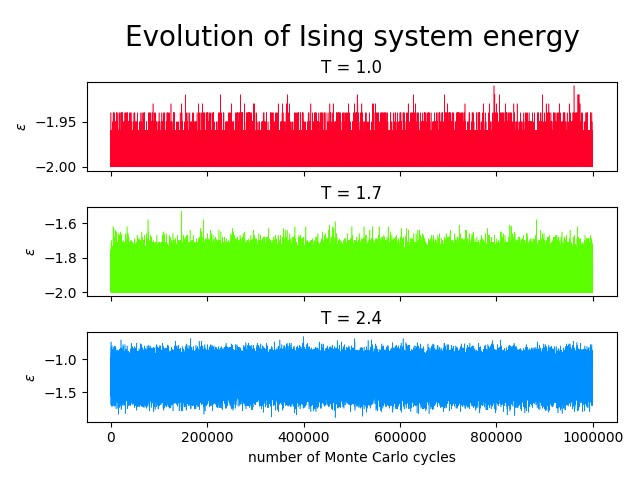
\includegraphics[scale=0.5]{../output/figures/experiment3/system_energy.png}
\caption{Evolution of the energy of the \(20\times20\) Ising system, starting from equilibrium.}\label{fig:experiment3_system_energy}
\end{figure}

\begin{figure}
\centering
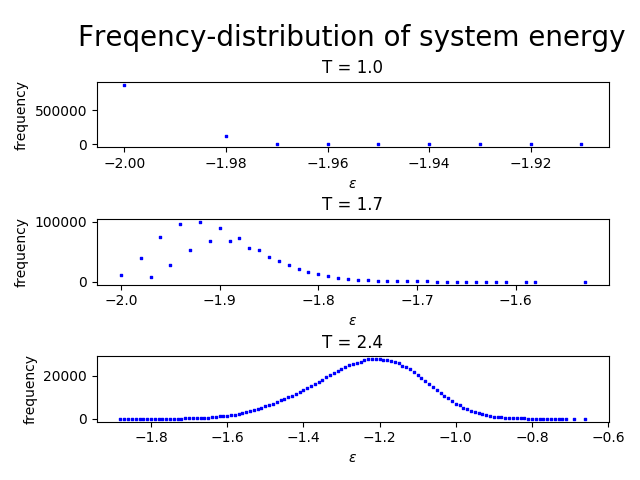
\includegraphics[scale=0.5]{../output/figures/experiment3/energy_distribution.png}
\caption{The distribution of energy states for the \(20\times20\) Ising system at equilibrium.}\label{fig:experiment3_energy_distribution}
\end{figure}

\begin{table}
\centering
\begin{tabular}{|c|c|c|}
\hline\rule{0pt}{0.32cm}
\(T\) & \(\sigma_\epsilon\)    \\\hline\rule{0pt}{0.32cm}
1.0   & \(7.9148\cdot10^{-3}\) \\\hline\rule{0pt}{0.32cm}
1.7   & \(4.9684\cdot10^{-2}\) \\\hline\rule{0pt}{0.32cm}
2.4   & \(1.4220\cdot10^{-1}\) \\\hline
\end{tabular}
\caption{Spread in energy during evolution from equilibrium of the \(20\times20\) system.}\label{tab:20by20_std_energy_evolution}
\end{table}

\subsection{Experiment 4}
The experimental results for the final experiment took a considerable amount of time to produce, which manifested itself in a smaller sample size of interesting data. The results are shown in figures \ref{fig:experiment4_energy_full}-\ref{fig:experiment4_magnetic_susceptibility}. There is quite a lot of instability within these figures as well as some conflicting results. Most notably, consider the temperature region about \(T\approx2.24\) in figure \ref{fig:experiment4_magnetic_susceptibility}: it is reasonable to assume the \(L=100\) curve should be closest to the exact result, however in this particular example it appears agrees with the tendencies of the \(L=40\) curve. Only making matters worse, both the \(L=60\) and \(L=80\) curves (which are seemingly "more accurate" than the \(L=40\) curve) show the complete opposite tendencies, meaning no convergence takes place.

Seeing that all the other experiments provided reasonable results, in addition to the fact that this experiment was the only one to be implement using parallel coding. It is not only possible, but probably the most reasonable explanation that some information has been handled incorrectly during the computation. This assertion is based on the observation that all the graphs seem to make abrupt and large fluctuations at the exact same temperatures. Moreover, the linear spacing of these temperature points is suspiciously similar to the division of the temperature range into four equally large temperature ranges during the parallel compuation. It is difficult to pinpoint exactly where the error stems from, especially because the code was built on the successful non-parallelized code used in previous experiments. The random generator used in the simulation is a standard Mersenne Twister, which could be one possibility of error.

The experimental data does not really indicate some sort of phase transition at all. Nevertheless, a critical temperature was estimated for the sake of the project. The following is a representation of what was intended to be done with a reasonable \(C_V(T)\).

\begin{figure}[h!]
\centering
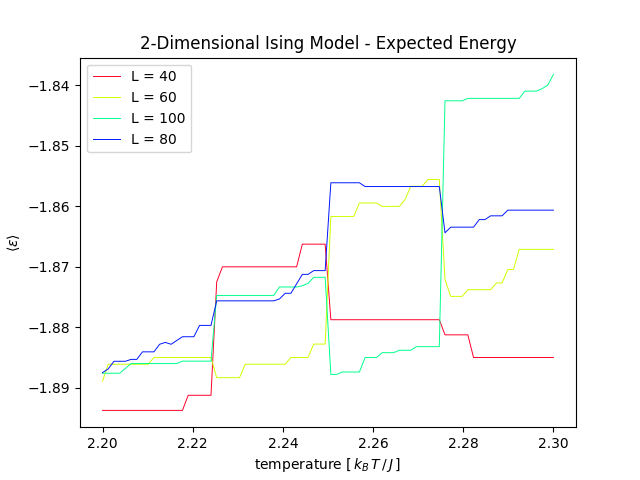
\includegraphics[scale=0.5]{../output/figures/experiment4/energy_full.png}
\caption{The energy of the Ising system as a function of temperature.}\label{fig:experiment4_energy_full}
\end{figure}

\begin{figure}[h!]
\centering
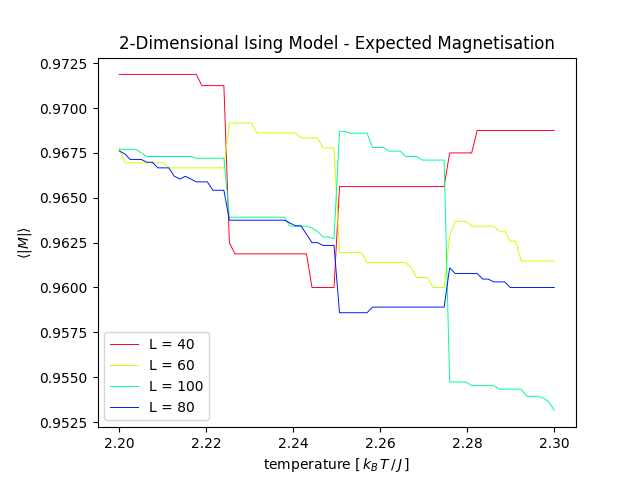
\includegraphics[scale=0.5]{../output/figures/experiment4/magnetisation_full.png}
\caption{The magnetisation of the Ising system as a function of temperature.}\label{fig:experiment4_magnetisation_full}
\end{figure}

\begin{figure}[h!]
\centering
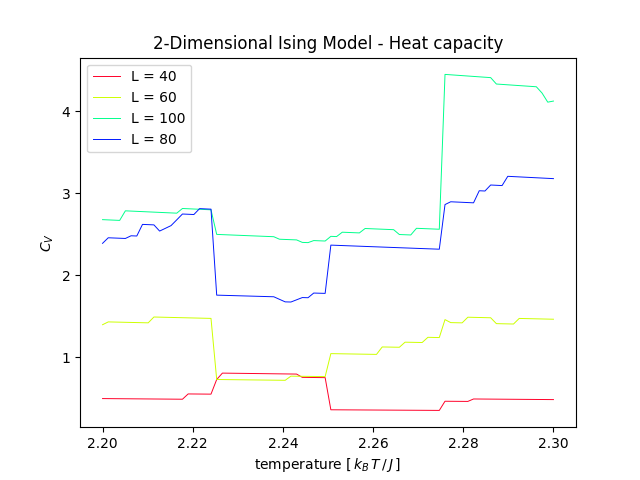
\includegraphics[scale=0.5]{../output/figures/experiment4/heat_capacity_full.png}
\caption{The heat capacity of the Ising system as a function of temperature.}\label{fig:experiment4_heat_capacity_full}
\end{figure}

\begin{figure}[h!]
\centering
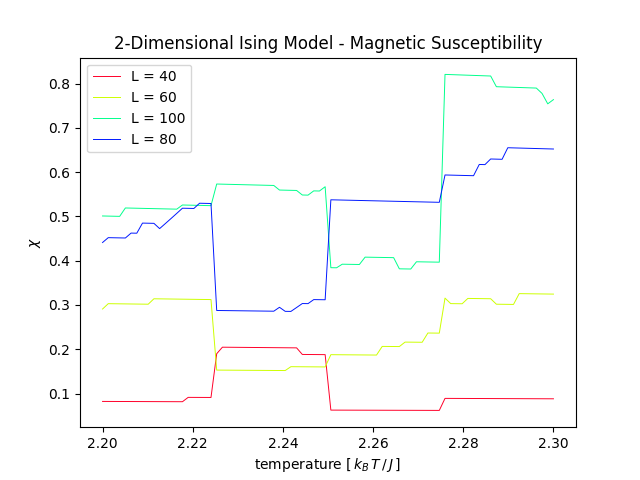
\includegraphics[scale=0.5]{../output/figures/experiment4/magnetic_susceptibility_full.png}
\caption{The magnetic susceptibility of the Ising system as a function of temperature.}\label{fig:experiment4_magnetic_susceptibility}
\end{figure}

The true critical temperature is about 2.27, however in ignorance of the true value the best estimate is the \(L=100\) curve. It so happens that all the thermodynamic properties of the \(L=100\) system undergo a critical shift for temperatures \(\approx2.28\), thus making this the most reasonable region for which a phase transition may occur. Now, there seems to be the most agreement (least contradiction) between the different systems in their estimate of heat capacity (figure \ref{fig:experiment4_heat_capacity_full}. Because heat capacity is expected to have a distinct maximum at the critical temperature (see figure \ref{fig:2by2_HeatCapacity_MagneticSusceptibility}), it is therefore the most reasonable figure to analyse. A zoomed-in version of the region is shown in figure \ref{fig:experiment4_heat_capacity_zoom}.

There is not particular polyomial form of \ref{fig:experiment4_heat_capacity_zoom}, so a simple second order polynomial was used as a linear regressor. The maximum of a concave down parabola \(ax^2+bx+c\), i.e. its vertex, is given by \(h=-b/2a\), thus making the estimation of the critical temperature simpler. An example of the polynomial fit is shown in figure \ref{fig:experiment4_polyfit}. Because different graphs behave somewhat differently in the high-temperature limit, slightly tailored temperature ranges were used in the regression. The resulting estimates for the critical temperature are shown in table \ref{tab:critical_temperatures}, the critical temperatures are plotted against the inverse lattice size in figure \ref{fig:experiment4_critical}. In conclusion, the final estimate for the critical temperature of the magnetic phase transition of the two-dimensional Ising model is \(\hat{T}_C=2.2754\), which is about 0.0064 away from the exact value. Note that no uncertainties have been discussed as the estimate is based on experimental data that really does not support the existence of a phase transition at all.

\begin{figure}[h!]
\centering
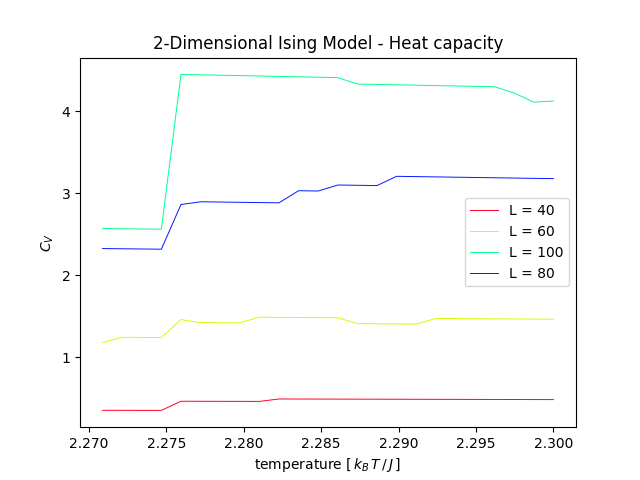
\includegraphics[scale=0.5]{../output/figures/experiment4/heat_capacity_zoom.png}
\caption{A zoomed-in version of figure \ref{fig:experiment4_heat_capacity_full}}\label{fig:experiment4_heat_capacity_zoom}
\end{figure}

\begin{figure}[h!]
\centering
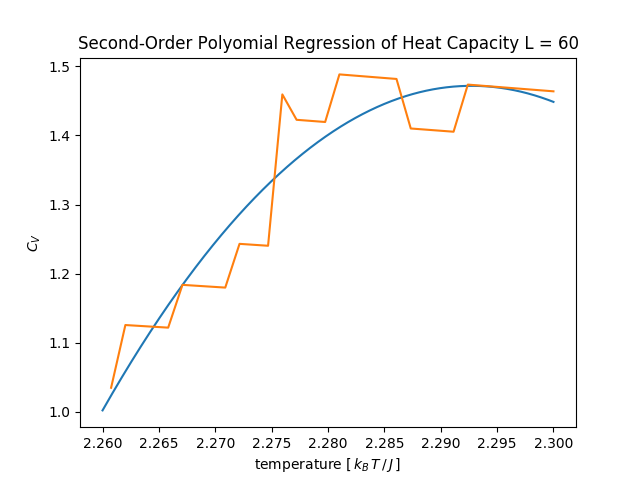
\includegraphics[scale=0.5]{../output/figures/experiment4/polyfit_60.png}
\caption{An example of the second-order polynomial fit of the heat capacity data.}\label{fig:experiment4_polyfit}
\end{figure}

\begin{table}
\centering
\begin{tabular}{|c|c|c|}
\hline\rule{0pt}{0.32cm}
\(L\) & \(T_C\) \\\hline\rule{0pt}{0.32cm}
 40 & 2.300606 \\\hline
 60 & 2.292721 \\\hline
 80 & 2.290087 \\\hline
100 & 2.283954 \\\hline
\end{tabular}
\caption{Critical temperatures for the Ising system.}\label{tab:critical_temperatures}
\end{table}

\begin{figure}[h!]
\centering
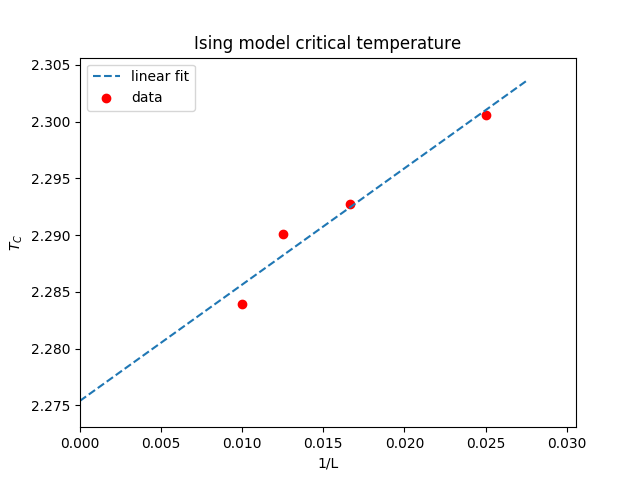
\includegraphics[scale=0.5]{../output/figures/experiment4/critical.png}
\caption{Critical temperatures for the Ising system as a function of the inverse of the lattice size.}\label{fig:experiment4_critical}
\end{figure}


\section{Discussion}
Overall the project has seen both major success and major failure in its attempt to simulate the Ising model. In experiment 1, the Metropolis algorithm provided a stable and reliable source of uncorrelated random states. Experiment 2 showed a clear converge towards equilibrium, regardless of whether the initial state was ordered or disordered, and for both high and low temperatures. The third experiment revealed the importance of lattice size, especially with regards to energy cut-off. It also quantified the fluctation spread of the system whilst in equilibrium with respect to temperature. And finally, the final experiment was more or less a complete failure as the experimental results were completely off the expected results.

With regards to experiment 1 there is actually a little room for improvement. The experiment only considered the \(2\times2\) system because it was solved exactly. This procedure is easily generalised as the exact solution to any two-dimensional lattice is known (see \citep{Onsager}). The same goes for experiment 2 and 3 in which only small lattices were analysed. Moreover, experiment 3 showed that the lattice size was even too small to capture the true energy distribution as it was cut off by a lacking number of available spins.

On the other hand, there is much room for improvement in the final experiment. Most of all, clearly some error was made during the implementation of the parallized computation. It is possible that the unstable nature of the results followed due to correlated "random" numbers from the Mersenne Twister, but this is only speculation at this point.

Although the final value is actually \emph{quite good}, it is unreasonable to place a firm belief in the findings. First of all, had it not been for the purpose of extracting a critical temperature, there never would have been a reason for analysing the data with respect to some form of phase transition. More importantly however, the regression analysis was incredibly tailored to the problem: most of the temperature data was ignored, the temperature range was tweaked to fit the data, etc.

\section{Conclusion}
In conclusion, the Metropolis algorithm has been shown to provide a stable, uncorrelated random set of states that are suitible for use in Monte Carlo integration. The Ising system used an average of \(10^5\) cycles to properly converge to the equilibrium state, regardless of the original state and regardless of temperature. Furthermore, the energy-distribution of the Ising system whist in equilibrium behaves fairly well according to an expected gaussian distribution. The accuracy of the energy-distribution improves with increasing lattice size, while also preventing cut-off errors due to lack of available spins. The project's final simulation, whose purpose was to estimate the critical temperature of the two-dimensional Ising model, failed to provide reasonable experimental data. The problem seems to be connected with the implementation of code parallelization as codes used in the previous experiments worked successfully.



\bibliographystyle{plain}
\bibliography{references.bib}


~
\clearpage
\appendix

\onecolumngrid
\section{Miscellaneous Material}\label{app:additional_material}
\subsection{All Possible Spin Configurations of The \(2\times2\) Ising Model}

\begin{table}[h!]
\centering
\caption{A display of all possible arrangements of the \(2\times2\) system. Each spin is allowed to occupy a spin-up state (\(\ua\)) or a spin-down state (\(\da\)).}\label{tab:2by2_microstates}
\scalebox{0.95}{
\begin{tabular}{M{2cm}|M{2cm}|M{2cm}|M{2cm} N}
\spinconfigmatrix{\da}{\da}{\da}{\da} &
\spinconfigmatrix{\da}{\da}{\da}{\ua} &
\spinconfigmatrix{\da}{\da}{\ua}{\da} &
\spinconfigmatrix{\da}{\da}{\ua}{\ua} &\\[1.5cm]\hline
%
\spinconfigmatrix{\da}{\ua}{\da}{\da} &
\spinconfigmatrix{\da}{\ua}{\da}{\ua} &
\spinconfigmatrix{\da}{\ua}{\ua}{\da} &
\spinconfigmatrix{\da}{\ua}{\ua}{\ua} &\\[1.5cm]\hline
%
\spinconfigmatrix{\ua}{\da}{\da}{\da} &
\spinconfigmatrix{\ua}{\da}{\da}{\ua} &
\spinconfigmatrix{\ua}{\da}{\ua}{\da} &
\spinconfigmatrix{\ua}{\da}{\ua}{\ua} &\\[1.5cm]\hline
%
\spinconfigmatrix{\ua}{\ua}{\da}{\da} &
\spinconfigmatrix{\ua}{\ua}{\da}{\ua} &
\spinconfigmatrix{\ua}{\ua}{\ua}{\da} &
\spinconfigmatrix{\ua}{\ua}{\ua}{\ua} &\\[1.5cm]
\end{tabular}
}
\end{table}

\subsection{Heat Capacity and Magnetic Susceptibility of The \(2\times2\) Ising Model}

\begin{figure}[h!]
\centering
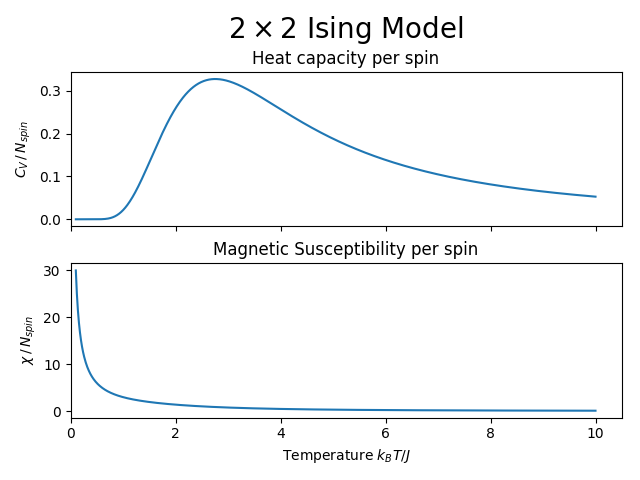
\includegraphics[scale=0.65]{../output/figures/2by2/heatcapacity_susceptibility.png}
\caption{\(2\times2\) Ising model.}\label{fig:2by2_HeatCapacity_MagneticSusceptibility}
\end{figure}


\clearpage
\subsection{All Possible Spin Configurations In The Flip One Tactic}

\begin{table}[h!]
\centering
\caption{A display of half of the possible arrangements of the spins involved in the flip one tactic. Each spin is allowed to occupy a spin-up state (\(\ua\)) or a spin-down state (\(\da\)). The central red spin is the spin to be flipped, the other half of the possible arrangements are the resulting flipped states.}\label{tab:2by2_microstates}
\scalebox{0.95}{
\begin{tabular}{M{2cm}|M{2cm}|M{2cm}|M{2cm} N}
\spinconfigmatrixneighbours{\ua}{\ua}{{\color{red}\ua}}{\ua}{\ua} &
\spinconfigmatrixneighbours{\ua}{\ua}{{\color{red}\ua}}{\ua}{\da} &
\spinconfigmatrixneighbours{\ua}{\ua}{{\color{red}\ua}}{\da}{\ua} &
\spinconfigmatrixneighbours{\ua}{\ua}{{\color{red}\ua}}{\da}{\da} &\\[1.5cm]\hline
%
\spinconfigmatrixneighbours{\ua}{\da}{{\color{red}\ua}}{\ua}{\ua} &
\spinconfigmatrixneighbours{\ua}{\da}{{\color{red}\ua}}{\ua}{\da} &
\spinconfigmatrixneighbours{\ua}{\da}{{\color{red}\ua}}{\da}{\ua} &
\spinconfigmatrixneighbours{\ua}{\da}{{\color{red}\ua}}{\da}{\da} &\\[1.5cm]\hline
%
\spinconfigmatrixneighbours{\da}{\ua}{{\color{red}\ua}}{\ua}{\ua} &
\spinconfigmatrixneighbours{\da}{\ua}{{\color{red}\ua}}{\ua}{\da} &
\spinconfigmatrixneighbours{\da}{\ua}{{\color{red}\ua}}{\da}{\ua} &
\spinconfigmatrixneighbours{\da}{\ua}{{\color{red}\ua}}{\da}{\da} &\\[1.5cm]\hline
%
\spinconfigmatrixneighbours{\da}{\da}{{\color{red}\ua}}{\ua}{\ua} &
\spinconfigmatrixneighbours{\da}{\da}{{\color{red}\ua}}{\ua}{\da} &
\spinconfigmatrixneighbours{\da}{\da}{{\color{red}\ua}}{\da}{\ua} &
\spinconfigmatrixneighbours{\da}{\da}{{\color{red}\ua}}{\da}{\da} &\\[1.5cm]
\end{tabular}
}
\end{table}





\end{document}